\documentclass[12pt,a4paper]{book}
\usepackage{pgf}
% \usepackage[condensed,math]{kurier}
% \usepackage[T1]{fontenc}
\usepackage{svg}
\usepackage{tikz}
\usepackage{stanli}
\usepackage{afterpage}
\usepackage{multirow}
\usepackage{subfig}
\usepackage{pgfpages}
\usepackage{svg}
\usepackage{rotating}
\usepackage{listings}
\usepackage{xcolor}

\lstset{
   language=Python,
   basicstyle=\ttfamily\small,
   numbers=left,
   numberstyle=\tiny\color{gray},
   frame=single,
   tabsize=4,
   breaklines=true,
   postbreak=\mbox{\textcolor{red}{$\hookrightarrow$}\space},
}


%\usepackage{times}


\pgfpagesdeclarelayout{boxed}
{
	\edef\pgfpageoptionborder{0pt}
}
{
	\pgfpagesphysicalpageoptions
	{%
		logical pages=1,%
	}
	\pgfpageslogicalpageoptions{1}
	{
		border code=\pgfsetlinewidth{2pt}\pgfstroke,%
		border shrink=\pgfpageoptionborder,%
		resized width=.9\pgfphysicalwidth,%
		resized height=.9\pgfphysicalheight,%
		center=\pgfpoint{.5\pgfphysicalwidth}{.5\pgfphysicalheight}%
	}%
}

\pgfpagesuselayout{boxed}


% Language setting
% Replace `english' with e.g. `spanish' to change the document language
\usepackage[english]{babel}

% Set page size and margins
% Replace `letterpaper' with `a4paper' for UK/EU standard size
\usepackage[a4paper,top=2cm,bottom=1.5cm,left=1.5cm,right=1.5cm,marginparwidth=1.75cm]{geometry}

% Useful packages
\usepackage{amsmath}
\usepackage{graphicx}
\usepackage[colorlinks=true, allcolors=blue]{hyperref}

\title{}
\author{}
\date{}

\begin{document}
	
	\newcommand{\subf}[2]{%
		{\small\begin{tabular}[t]{@{}c@{}}
				#1\\#2
		\end{tabular}}%
	}
	
	\begin{titlepage}
		\begin{center}
			\vspace*{3cm}
			
			\Huge
			\textbf{CSL7670 : Fundamentals of \\Machine Learning}
			
			\vspace{0.3cm}
			\Huge
			Lab Report
			
			\vspace{0.8cm}
			\large
			
			%INSTRUCTED BY: MRS. A.A.S.KAUSHLYA
			
			
			\vspace{0.5cm}
			\LARGE
			
			
			\vspace{1.5cm}
			
			\textbf{}
            
\includegraphics[width=0.4\textwidth]{IITJ Logo__Small.jpeg}
			
			\vfill
			
			
			
			\vspace{0.8cm}
			
			
			
			\Large
			
			
			
			
		\end{center}
		\Large
		\begin{tabbing}
			\hspace*{1em}\= \hspace*{8em} \= \kill % set the tabbings
			\> Name:\>  \textbf{YOUR NAME} \\
                \> Roll Number:\>  \textbf{YOUR Roll Number} \\
                 \> Program:\>  \textbf{Your Program} \\
					\end{tabbing}
		
	\end{titlepage}
	
\chapter{Lab-1}
\section{Objective}
Objective of this assignment is to brush up on the programming skills required for ML. This assignment contains 16 problems. So accordingly, prepare appropriate inputs or input files as required and submit a detailed Python codes.

\section{Problem-1}
Lists and Loops: Write a Python function that takes a list of integers as input and returns the sum of all even numbers in the list.\\

\textbf{Solution 1: }
\lstinputlisting[style=mystyle]{Lab-1/src/Prob-1.py}

\textbf{Output 1: }
\lstinputlisting[style=mystyle]{Lab-1/Prob_sol-1.txt}\\

\section{Problem-2}
List Comprehension: Given a list of words, create a new list containing the length of each word using list comprehension.\\\\

\textbf{Solution 2: }
\lstinputlisting[style=mystyle]{Lab-1/src/Prob-2.py}

\textbf{Output 2: }
\lstinputlisting[style=mystyle]{Lab-1/Prob_sol-2.txt}\\

\section{Problem-3}
NumPy Array Operations: Given two NumPy arrays arr1 = np.array([1,2, 3]) and arr2 = np.array([4, 5, 6]), perform element-wise multiplication and store the result in a new array.\\

\textbf{Solution 3: }
\lstinputlisting[style=mystyle]{Lab-1/src/Prob-3.py}

\textbf{Output 3: }
\lstinputlisting[style=mystyle]{Lab-1/Prob_sol-3.txt}\\

\section{Problem-4}
NumPy Array Slicing: Given a NumPy array data = np.arange(1, 21), use array slicing to extract elements from index 5 to index 15.\\

\textbf{Solution 4): }
\lstinputlisting[style=mystyle]{Lab-1/src/Prob-4.py}

\textbf{Output 4:}
\lstinputlisting[style=mystyle]{Lab-1/Prob_sol-4.txt}\\

\section{Problem-5}
Data Visualization with Matplotlib: Using Matplotlib, create a line plot to visualize the trend of a stock’s closing price over ten days (random data can be used).\\

\textbf{Solution 5: }
\lstinputlisting[style=mystyle]{Lab-1/src/Prob-5.py}

\begin{figure}[ht]
\centering
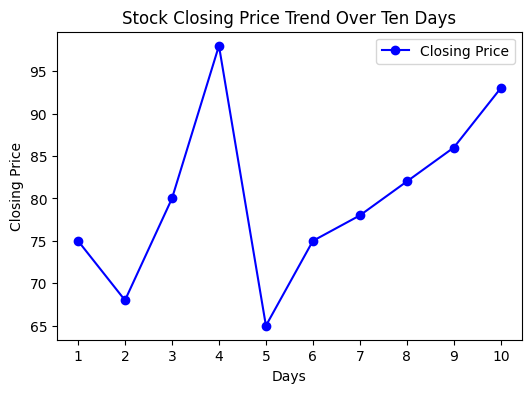
\includegraphics[width=7.5cm]{Lab-1/data/prob-5.png}
\caption{Line plot determining the stock closing price.}
\label{fig:sample}
\end{figure}

\section{Problem-6}
Data Cleaning with Pandas:** Given a Pandas DataFrame with a column containing missing values, write a Python function to replace those missing values with the mean of that column.\\

\textbf{Solution 6: }
\lstinputlisting[style=mystyle]{Lab-1/src/Prob-6.py}

\textbf{Output 6: }
\lstinputlisting[style=mystyle]{Lab-1/Prob_sol-6.txt}\\

\section{Problem-7}
Pandas DataFrame Filtering: Using Pandas, filter a DataFrame to only include rows where the ’age’ column is greater than 30 and the ’gender’ column is ’female’.\\

\textbf{Solution 7: }
\lstinputlisting[style=mystyle]{Lab-1/src/Prob-7.py}

\textbf{Output 7: }
\lstinputlisting[style=mystyle]{Lab-1/Prob_sol-7.txt}\\

\section{Problem-8}
Pandas Grouping: Given a DataFrame with columns ’Country’ and ’Population’, use Pandas to group the data by ’Country’ and calculate the average population for each country.\\

\textbf{Solution 8: }
\lstinputlisting[style=mystyle]{Lab-1/src/Prob-8.py}

\textbf{Output 8:}
\lstinputlisting[style=mystyle]{Lab-1/Prob_sol-8.txt}\\

\section{Problem-9}
Data Visualization with Seaborn: Using Seaborn, create a box plot to visualize the distribution of ages for different ’Species’ in a DataFrame.\\

\textbf{Solution 9: }
\lstinputlisting[style=mystyle]{Lab-1/src/Prob-9.py}

\begin{figure}[ht]
\centering
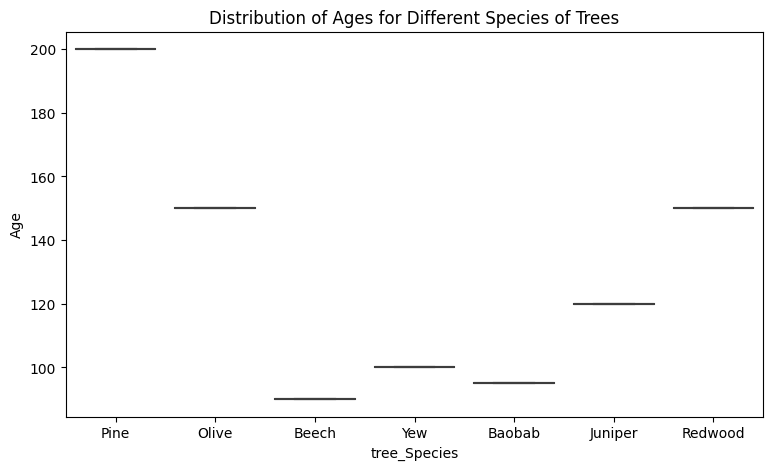
\includegraphics[width=9cm]{Lab-1/data/prob-9.png}
\caption{Box Plot showing the different species of tree.}
\label{fig:sample}
\end{figure}

\FloatBarrier

\section{Problem-10}
Data Manipulation with Pandas: Given a Pandas DataFrame containing columns ’Sales’ and ’Expenses’, create a new column ’Profit’ that calculates the profit as ’Sales’ minus ’Expenses’.\\

\textbf{Solution 10: }
\lstinputlisting[style=mystyle]{Lab-1/src/Prob-10.py}

\textbf{Output 10: }
\lstinputlisting[style=mystyle]{Lab-1/Prob_sol-10.txt}\\

\section{Problem-11}
Dictionary Manipulation: Given a dictionary phonebook containing names as keys and phone numbers as values, write a function to find and return the name(s) of the person(s) with the maximum phone number(s).\\

\textbf{Solution 11: }
\lstinputlisting[style=mystyle]{Lab-1/src/Prob-11.py}

\textbf{Output 11: }
\lstinputlisting[style=mystyle]{Lab-1/Prob_sol-11.txt}\\

\section{Problem-12}
Functions and Recursion: Write a recursive Python function to calculate the factorial of a given positive integer.\\\\

\textbf{Solution 12: }
\lstinputlisting[style=mystyle]{Lab-1/src/Prob-12.py}

\textbf{Output 12:}
\lstinputlisting[style=mystyle]{Lab-1/Prob_sol-12.txt}\\

\section{Problem-13}
File Handling: Read a text file named “data.txt” that contains one number per line. Write a Python script to calculate the sum of all the numbers and print the result.\\

\textbf{Solution 13: }
\lstinputlisting[style=mystyle]{Lab-1/src/Prob-13.py}

\textbf{Output 13:}
\lstinputlisting[style=mystyle]{Lab-1/Prob_sol-13.txt}\\

\section{Problem-14}
Object-Oriented Programming: Create a class Rectangle with attributeswidth and height, and methods to calculate the area and perimeter. Test the class by creating objects and performing calculations.\\

\textbf{Solution 14: }
\lstinputlisting[style=mystyle]{Lab-1/src/Prob-14.py}

\textbf{Output 14:}
\lstinputlisting[style=mystyle]{Lab-1/Prob_sol-14.txt}\\

\section{Problem-15}
Numpy Array Manipulation: Create a 3×3 identity matrix using NumPy and then convert it into a 1D array.\\

\textbf{Solution 15: }
\lstinputlisting[style=mystyle]{Lab-1/src/Prob-15.py}

\textbf{Output 15:}
\lstinputlisting[style=mystyle]{Lab-1/Prob_sol-15.txt}\\

\section{Problem-16}
Data Visualization with Matplotlib: Using Matplotlib, create a bar chart to compare the average scores of students in three different subjects.\\

\textbf{Solution 16:}
\lstinputlisting[style=mystyle]{Lab-1/src/Prob-16.py}

\begin{figure}[ht]
\centering
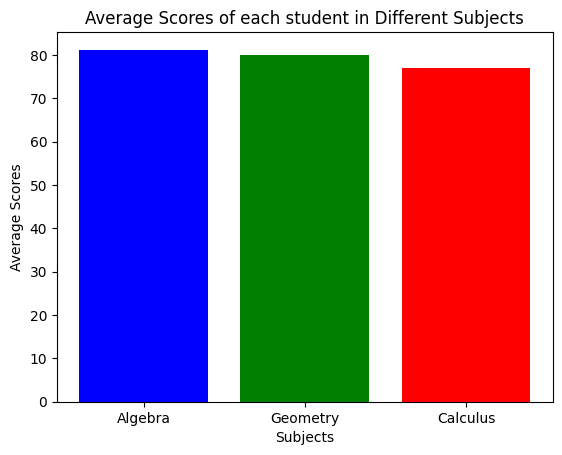
\includegraphics[width=6cm]{Lab-1/data/prob-16.png}
\caption{Histogram showing the avg scores of each student.}
\label{fig:sample}
\end{figure}	
\chapter{Lab-2}
\section{Objective}
The main Objective of this assignment is to get familiarity with K-NN. The first problem is on (Handwritten Digit Classification) Use the code provided for classifying the handwritten digits of the MNIST dataset. Read and understand the code.

\section{Problem-1(a)}
Modify the code so that it uses L1-distance instead of the default L2-distance (Eucleadean).

\textbf{Solution 1(a): }
\lstinputlisting[style=mystyle]{Lab-2/MNIST_1.py}\\

\textbf{Output 1(a): }
\lstinputlisting[style=mystyle]{Lab-2/MNIST_sol_1.txt}\\

\section{Problem-2(a)}
Display results by showing the image, actual label, and predicted label. 

\textbf{Solution 2(a): }
\lstinputlisting[style=mystyle]{Lab-2/MNIST_2.py}\\

\textbf{Output 2(a): }

\begin{figure}[ht]
\centering
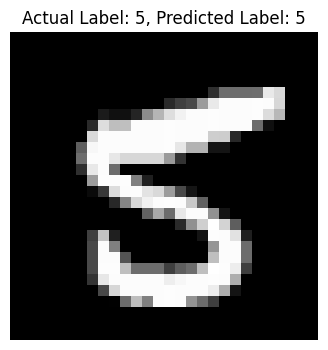
\includegraphics[width=3.5cm]{Lab-2/data/5.png}
\caption{Image generated for label 5.}
\label{fig:sample}
\end{figure}

\FloatBarrier

\begin{figure}[ht]
\centering
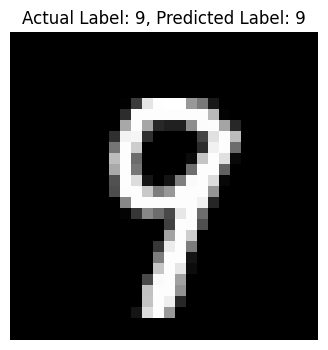
\includegraphics[width=3.5cm]{Lab-2/data/9.png}
\caption{Image sample generated for label 9.}
\label{fig:sample}
\end{figure}

\FloatBarrier

\begin{figure}[ht]
\centering
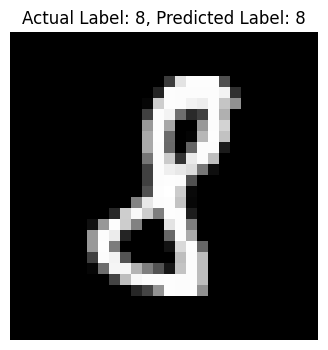
\includegraphics[width=3.5cm]{Lab-2/data/8.png}
\caption{Image sample generated for label 8.}
\label{fig:sample}
\end{figure}

\FloatBarrier

\begin{figure}[ht]
\centering
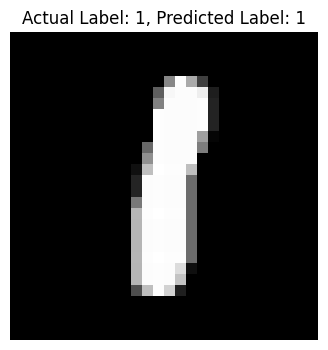
\includegraphics[width=3.5cm]{Lab-2/data/1.png}
\caption{Image sample generated for label 1.}
\label{fig:sample}
\end{figure}

\FloatBarrier

\section{Problem-3(a)}
Find out a few samples where the predicted label is incorrect.\\

\textbf{Solution 3(a): }
\lstinputlisting[style=mystyle]{Lab-2/MNIST_3.py}\\

\textbf{Output 3(a): }

\begin{figure}[ht]
\centering
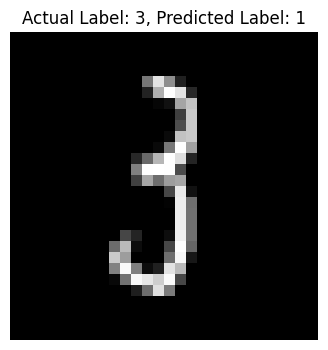
\includegraphics[width=3.5cm]{Lab-2/data/3_1.png}
\caption{Mismatched Image sample of actual label 3 with predicted label 1.}
\label{fig:sample}
\end{figure}

\FloatBarrier

\begin{figure}[ht]
\centering
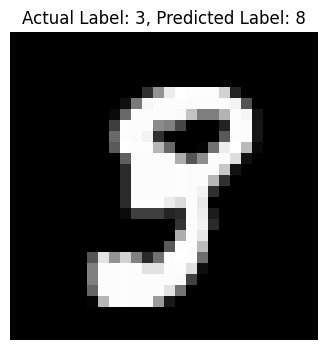
\includegraphics[width=3.5cm]{Lab-2/data/3_9.png}
\caption{Mismatched Image sample of actual label 3 with predicted label 8.}
\label{fig:sample}
\end{figure}

\FloatBarrier

\begin{figure}[ht]
\centering
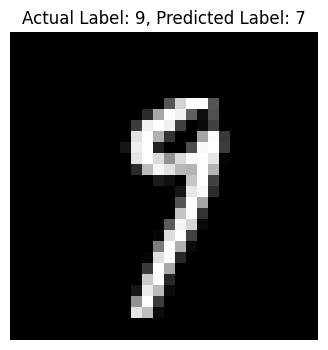
\includegraphics[width=3.5cm]{Lab-2/data/9_7.png}
\caption{Mismatched Image sample of actual label 9 with predicted label 7.}
\label{fig:sample}
\end{figure}

\FloatBarrier

\section{Objective}
The second problem is on the (Apple vs Orange) classification. You are given a K-NN code for Apple vs Orange problem. Please read and understand the code. Now perform the following tasks:

\section{Problem-1(b)}
Synthetically increase the dataset size to 50 samples.\\\\

\textbf{Solution 1(b): }
\lstinputlisting[style=mystyle]{Lab-2/KNN_1.py}\\

\textbf{Output 1(b): }
\lstinputlisting[style=mystyle]{Lab-2/KNN_sol_1.txt}\\

\lstinputlisting[style=mystyle]{Lab-2/KNN_5.py}
\lstinputlisting[style=mystyle]{Lab-2/KNN_sol_7.txt}

\section{Problem-2(b)}
Edit the code so that random 80 percentage, 10 percentage, and 10 percentage samples are used for training, testing, and validation respectively.\\

\textbf{Solution 2(b): }
\lstinputlisting[style=mystyle]{Lab-2/KNN_2.py}\\

\textbf{Output 2(b): }
\lstinputlisting[style=mystyle]{Lab-2/KNN_sol_2.txt}\\

\section{Problem-3(b)}
Change the value of K to 3, 5, and 7 and compare the validation set and test set results.

\textbf{Solution 3(b): }
\lstinputlisting[style=mystyle]{Lab-2/KNN_3.py}\\

\textbf{Output 3(b): }
\lstinputlisting[style=mystyle]{Lab-2/KNN_sol_3.txt}\\

\section{Problem-4(b)}
Write a code that draws confusion matrices for different K.

\textbf{Solution 4(b): }
\lstinputlisting[style=mystyle]{Lab-2/KNN_4.py}\\

\textbf{Output 4(b): }
\lstinputlisting[style=mystyle]{Lab-2/KNN_sol_4.txt}\\

\begin{figure}[ht]
\centering
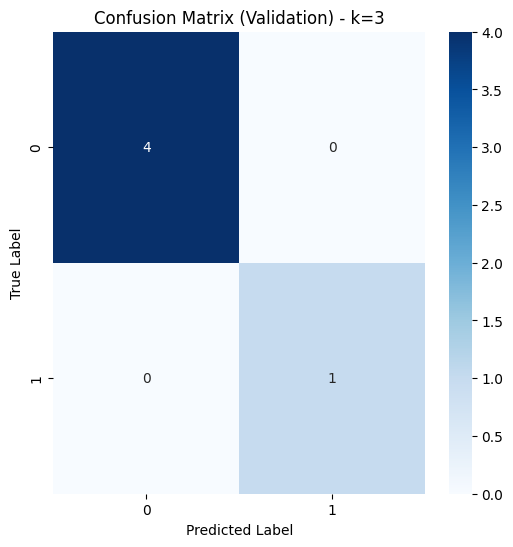
\includegraphics[width=5.7cm]{Lab-2/data/k_3.png}
\caption{Confusion Matrix ( Validation ) for k=3.}
\label{fig:sample}
\end{figure}

\FloatBarrier

\lstinputlisting[style=mystyle]{Lab-2/KNN_sol_5.txt}\\

\begin{figure}[ht]
\centering
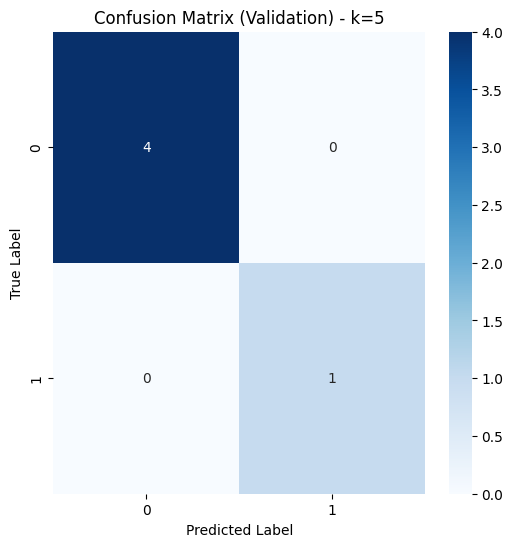
\includegraphics[width=5.7cm]{Lab-2/data/k_5.png}
\caption{Confusion Matrix ( Validation ) for k=5.}
\label{fig:sample}
\end{figure}

\FloatBarrier

\lstinputlisting[style=mystyle]{Lab-2/KNN_sol_6.txt}
\begin{figure}[ht!]
\centering
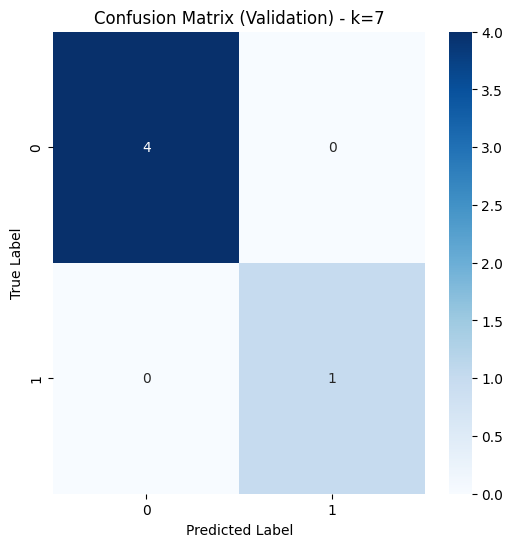
\includegraphics[width=5.7cm]{Lab-2/data/k_7.png}
\caption{Confusion Matrix ( Validation ) for k=7.}
\label{fig:sample}
\end{figure}
	






\end{document}

	
	
	
